\documentclass{article}
\usepackage[utf8]{inputenc} %кодировка
\usepackage[T2A]{fontenc}
\usepackage[english,russian]{babel} %русификатор 
\usepackage{mathtools} %библиотека матеши
\usepackage[left=1cm,right=1cm,top=2cm,bottom=2cm,bindingoffset=0cm]{geometry} %изменение отступов на листе
\usepackage{amsmath}
\usepackage{graphicx} %библиотека для графики и картинок
\graphicspath{}
\DeclareGraphicsExtensions{.pdf,.png,.jpg}
\usepackage{subcaption}
\usepackage{pgfplots}
\usepackage{float}
\usepackage{listings}
\usepackage{hyperref}

\lstset{
    language=Java,
    frame=single,
    breaklines=true,
    numbers=left, % нумерация строк
    caption={Пример Java кода}, 
    label={lst:java_example}
}

\begin{document}
% НАЧАЛО ТИТУЛЬНОГО ЛИСТА
\begin{center}
    \Large
    Федеральное государственное автономное \\
    образовательное учреждение высшего образования \\ 
    «Научно-образовательная корпорация ИТМО»\\
    \vspace{0.5cm}
    \large
    Факультет программной инженерии и компьютерной техники \\
    Направление подготовки 09.03.04 Программная инженерия \\
    \vspace{1cm}
    \Large
    \textbf{Отчёт по лабораторной работе №3} \\
    По дисциплине «Вычислительная математика» (4 семестр)\\
    \large
    \vspace{8cm}

    \begin{minipage}{.33\textwidth}
    \end{minipage}
    \hfill
    \begin{minipage}{.4\textwidth}
    
        \textbf{Студент}: \vspace{.1cm} \\
        \ Дениченко Александр P3212\\
        \textbf{Практик}:  \\
        \ Наумова Надежда Александровна
    \end{minipage}
    \vfill
Санкт-Петербург\\ 2024 г.
\end{center}
\pagestyle{empty}
% КОНЕЦ ТИТУЛЬНОГО ЛИСТА 
\newpage
\pagestyle{plain}
\section{Цель работы}
Найти приближенное значение определенного интеграла с требуемой точностью различными численными методами.
\[\text{Вариант} - 8\]
\section{Вычислительная часть}
1. Вычислить интеграл, приведенный в таблице 1, точно.\\
2. Вычислить интеграл по формуле Ньютона – Котеса при n = 6.\\
3. Вычислить интеграл по формулам средних прямоугольников, трапеций и Симпсона при n = 10 .\\
4. Сравнить результаты с точным значением интеграла.\\
5. Определить относительную погрешность вычислений для каждого метода.\\
6. В отчете отразить последовательные вычисления.\\
\\
\textbf{Интеграл по варианту:}
\[\int_{2}^{3}3x^3-2x^2-7x-8\]
\textbf{Точное вычисление интеграла:}
\[\int_{2}^{3}3x^3-2x^2-7x-8 = \left(\frac{3x^4}{4} - \frac{2x^3}{3} - \frac{7x^2}{2}-8x\right)\biggr|_2^3 = \frac{243}{4} - \frac{301}{6} = \frac{127}{12} \approx 10.583\]
\textbf{Вычисление по формуле Ньютона – Котеса:}\\ \\
Берём n=6, тогда коэффициенты Котеса для равноотстоящих узлов:
\[c_6^0 = c_6^6 = \frac{42(b-a)}{840}\]
\[c_6^1 = c_6^5 = \frac{216(b-a)}{840}\]
\[c_6^2 = c_6^4 = \frac{27(b-a)}{840}\]
\[c_6^3= \frac{272(b-a)}{840}\]
Границы известны a=2; b=3:
\[c_6^0 = c_6^6 = \frac{42}{840}\]
\[c_6^1 = c_6^5 = \frac{216}{840}\]
\[c_6^2 = c_6^4 = \frac{27}{840}\]
\[c_6^3= \frac{272}{840}\]
Найдём шаг разбиения:
\[h = \frac{3-2}{6} = \frac{1}{6}\]
Запишем определенный интеграл в виде:
\[\int_{2}^{3}3x^3-2x^2-7x-8 = c_6^0\cdot f(a) 
+ c_6^1\cdot f(a+\frac{1}{6})
+ c_6^2\cdot f(a+\frac{2}{6}) 
+ c_6^3\cdot f(a+\frac{3}{6})
+ c_6^4\cdot f(a+\frac{4}{6})
+ c_6^5\cdot f(a+\frac{5}{6})
+ c_6^6\cdot f(b)=
\]
\[= \frac{42}{840}\cdot f(2) 
+ \frac{216}{840}\cdot f(2+\frac{1}{6})
+ \frac{27}{840}\cdot f(2+\frac{2}{6}) 
+ \frac{272}{840}\cdot f(2+\frac{3}{6})
+ \frac{27}{840}\cdot f(2+\frac{4}{6})
+ \frac{216}{840}\cdot f(2+\frac{5}{6})
+ \frac{42}{840}\cdot f(3)\approx 10.617
\]
Относительная погрешность:
\[\epsilon = \frac{|10.617 - 10.583|}{10.583}\cdot 100 = 0.32\%\]
\\
\textbf{Вычисление по формуле прямоугольников со средними высотами:}\\ \\
По условия дано n = 10, тогда делим отрезок интегрирования на 10 равных частей по формуле:
\[h=\frac{b-a}{n} = \frac{3-2}{10} = 0.1\]
По формуле средних прямоугольников:
\[I = h\sum_{i=1}^{n}y_{i-\frac{1}{2}}\]
\begin{table}[H]
    \centering
    \begin{tabular}{|c|c|c|c|c|c|c|c|c|c|c|c|}
        \hline
        $i$ & 0 & 1 & 2 & 3 & 4 & 5 & 6& 7& 8& 9& 10\\
        \hline
        $x_i$ & 2 & 2,1 & 2,2& 2,3& 2,4& 2,5& 2,6& 2,7& 2,8& 2,9& 3\\
        \hline
        $y_i$ &-6& -3.737& -1.136& 1.821& 5.152& 8.875& 13.008& 17.569& 22.576& 28.047& 34 \\
        \hline
        $x_{i-1/2}$ & & 2.05 & 2.15 & 2.25 & 2.35 & 2.45& 2.55& 2.65& 2.75& 2.85& 2.95 \\
        \hline
        $y_{i-1/2}$ & & -4.9096& -2.4799& 0.2969& 3.4386& 6.9634& 10.8891& 15.2339& 20.0156& 25.2524& 30.9621 \\
        \hline
        \end{tabular}
        \caption{Приближенное вычисление интеграла методом средних прямоугольников}
        \label{tab:midpoint_approximation}  
\end{table}
Подсчёт:
\[I = 0.1\cdot (-4.9096 -2.4799+ 0.2969+ 3.4386+ 6.9634+ 10.8891+ 15.2339+ 20.0156+ 25.2524+ 30.9621) = 10.8737\]
Относительная погрешность:
\[\epsilon = \frac{|10.8737 - 10.583|}{10.583}\cdot 100 = 2.75\%\]
\\
\textbf{Вычисление методом трапеций:}\\ \\
По условия дано n = 10, тогда делим отрезок интегрирования на 10 равных частей по формуле:
\[h=\frac{b-a}{n} = \frac{3-2}{10} = 0.1\]
По формуле трапеций:
\[I = h\cdot \left(\frac{y_0+y_{10}}{2}+\sum_{i=1}^{n-1}y_i\right)\]
\begin{table}[H]
    \centering
    \begin{tabular}{|c|c|c|c|c|c|c|c|c|c|c|c|}
        \hline
        $i$ & 0 & 1 & 2 & 3 & 4 & 5 & 6& 7& 8& 9& 10\\
        \hline
        $x_i$ & 2 & 2,1 & 2,2& 2,3& 2,4& 2,5& 2,6& 2,7& 2,8& 2,9& 3\\
        \hline
        $y_i$ &-6& -3.737& -1.136& 1.821& 5.152& 8.875& 13.008& 17.569& 22.576& 28.047& 34 \\
        \hline
        \end{tabular}
        \caption{Приближенное вычисление интеграла методом трапеций}
        \label{tab:midpoint_approximation}  
\end{table}
Подсчёт:
\[I = 0.1\cdot \left(\frac{-6+43}{2}+(-6-3.737-1.136+1.821+5.152+8.875+13.008+17.569+22.576 +28.047)\right) = 10.0175\]
Относительная погрешность:
\[\epsilon = \frac{|10.0175 - 10.583|}{10.583}\cdot 100 = 5.34\%\]
\\
\textbf{Вычисление методом Симпсона:}\\ \\
По условия дано n = 10, тогда делим отрезок интегрирования на 10 равных частей по формуле:
\[h=\frac{b-a}{n} = \frac{3-2}{10} = 0.1\]
По формуле Симпсона:
\[I = \frac{h}{3}(y_0+ 4\cdot(y_1 + y_3+ y_5+ y_7+ y_9)+2\cdot(y_2 + y_4+ y_6+ y_8) + y_{10}) = \] 
\begin{table}[H]
    \centering
    \begin{tabular}{|c|c|c|c|c|c|c|c|c|c|c|c|}
        \hline
        $i$ & 0 & 1 & 2 & 3 & 4 & 5 & 6& 7& 8& 9& 10\\
        \hline
        $x_i$ & 2 & 2,1 & 2,2& 2,3& 2,4& 2,5& 2,6& 2,7& 2,8& 2,9& 3\\
        \hline
        $y_i$ &-6& -3.737& -1.136& 1.821& 5.152& 8.875& 13.008& 17.569& 22.576& 28.047& 34 \\
        \hline
        \end{tabular}
        \caption{Приближенное вычисление интеграла методом Симпсона}
        \label{tab:midpoint_approximation}  
\end{table}

\[= \frac{0.1}{3}(-6+ 4\cdot(-3.737 + 1.821+ 8.875+ 17.569+ 28.047)+2(-1.136 + 5.152+ 13.008+ 22.576) + 34) = 10.5833\]\\
Относительная погрешность:
\[\epsilon = \frac{|10.5833 - 10.583|}{10.583}\cdot 100 = 0.0028\%\]
\section{Машинная реализация}

\begin{lstlisting}[language=Java, caption={Первый узел валидации}]
private CalculateError isValidInterval(RequestFuncUser requestFuncUser) {
    ArrayList<Double> kritPoints = new Functions().getErrPoints((int) requestFuncUser.getTypeFunc());
    if(requestFuncUser.getA()>requestFuncUser.getB()){
        double tmp = requestFuncUser.getA();
        requestFuncUser.setA(requestFuncUser.getB());
        requestFuncUser.setB(tmp);
    }
    Double a = requestFuncUser.getA();
    Double b = requestFuncUser.getB();
    Functions functions = new Functions();

    if(a.equals(b)) {
        return CalculateError.INCORRECT_BOUNDS_NULL_S;
    }
    for (Double point : kritPoints) {
        logger.info("point > a: "+(point>a)+"; point<b: "+(point<b));
        if (point.equals(a) && !Double.isNaN(functions.f_dx(a, (int) requestFuncUser.getTypeFunc()))
                && Double.isFinite(functions.f_dx(a, (int) requestFuncUser.getTypeFunc()))) {
            requestFuncUser.setA(a + 0.0000001);
        } else if (point.equals(b) && !Double.isNaN(functions.f_dx(b, (int) requestFuncUser.getTypeFunc()))
                && Double.isFinite(functions.f_dx(b, (int) requestFuncUser.getTypeFunc()))) {
            requestFuncUser.setB(b - 0.0000001);
        }else if (Double.isNaN(functions.f_dx(a, (int) requestFuncUser.getTypeFunc())) ||
                Double.isNaN(functions.f_dx(b, (int) requestFuncUser.getTypeFunc()))
                || Double.isInfinite(functions.f_dx(a, (int) requestFuncUser.getTypeFunc()))
                || Double.isInfinite(functions.f_dx(b, (int) requestFuncUser.getTypeFunc()))) {
            return CalculateError.INCORRECT_BOUNDS_INT_ERR;
        }
        if(point>a && point<b && (Double.isNaN(functions.f_dx(point, (int) requestFuncUser.getTypeFunc()))
                || Double.isInfinite(functions.f_dx(point, (int) requestFuncUser.getTypeFunc())) )){
            logger.warn("somnitelno no okey");
        }
    }
    logger.info("f_dx(a): "+functions.f_dx(a, (int) requestFuncUser.getTypeFunc())+"; f_dx(b): "+functions.f_dx(b, (int) requestFuncUser.getTypeFunc()));
    return null;
} 
\end{lstlisting}

\begin{lstlisting}[language=Java, caption={Второй узел валидации}]
if(critInterval.isEmpty()){
    mathMethod = getMethod((int) pointRequest.getMethod(), pointRequest);
    mathMethod.calculate();
    tmp = mathMethod.getAnswer().outAnswer();
}else {
    double a = pointRequest.getA();
    double b = pointRequest.getB();
    double crit1 = critInterval.get(0);
    double crit2 = critInterval.get(1);
    if (a < crit1 && b > crit2) {
        RequestFuncUser interval1 = pointRequest.clone();
        interval1.setB(crit1);
        logger.info(interval1.toString());

        RequestFuncUser interval2 = pointRequest.clone();
        interval2.setA(crit2);
        logger.info(interval2.toString());

        MathMethod mathMethod1 = getMethod((int) interval1.getMethod(), interval1);
        MathMethod mathMethod2 = getMethod((int) interval2.getMethod(), interval2);


        mathMethod1.calculate();
        mathMethod2.calculate();
        logger.info(mathMethod1.answerInfo.toString());
        logger.info(mathMethod2.answerInfo.toString());

        double e = mathMethod1.answerInfo.e;
        double ans = mathMethod1.answerInfo.answer + mathMethod2.answerInfo.answer;
        double r = (mathMethod1.answerInfo.r + mathMethod2.answerInfo.r)/2;
        long n = mathMethod1.answerInfo.n + mathMethod2.answerInfo.n;
        AnswerInfo answerInfo = new AnswerInfo(e, ans, ans, r, n);
        if(Math.abs(interval1.getA()) == Math.abs(interval2.getB())){
            answerInfo = new AnswerInfo(0, 0, 0, 0, 0);
        }
        tmp = answerInfo.outAnswer();
    } else if (a >= crit1 && b <= crit2) {
        AnswerInfo answerInfo = new AnswerInfo(0, 0, 0, 0, 0);
        tmp = answerInfo.outAnswer();
    } else if (a >= crit1 && a <= crit2 && b > crit2) {
        RequestFuncUser interval1 = pointRequest.clone();
        interval1.setA(crit2);
        MathMethod mathMethod1 = getMethod((int) interval1.getMethod(), interval1);
        mathMethod1.calculate();
        logger.info(mathMethod1.answerInfo.toString());
        tmp = mathMethod1.answerInfo.outAnswer();
    } else if (a < crit1 && b <= crit2 && b >= crit1) {
        RequestFuncUser interval1 = pointRequest.clone();
        interval1.setB(crit1);
        MathMethod mathMethod1 = getMethod((int) interval1.getMethod(), interval1);
        mathMethod1.calculate();
        logger.info(mathMethod1.answerInfo.toString());
        tmp = mathMethod1.answerInfo.outAnswer();
    } else if ((b < crit1)||(a > crit2)) {
        mathMethod = getMethod((int) pointRequest.getMethod(), pointRequest);
        mathMethod.calculate();
        tmp = mathMethod.getAnswer().outAnswer();
    } else {
        AnswerInfo answerInfo = new AnswerInfo(0, 0, 0, 0, 0);
        tmp = answerInfo.outAnswer();
    }
}
    \end{lstlisting}

\begin{lstlisting}[language=Java, caption={Метод средних прямоугольников}]
public void calculate() {
    if (a > b) {
        double tmp = a;
        a = b;
        b = tmp;
    }

    double step, sum, r = e + 1;
    long n = 4;
    double currAns = 0, prevAns = 0;

    while (r > e){
        step = (b - a) / n;
        sum = 0;
        for (int i = 0; i < n; i++) {
            double aNew = a + step / 2 + step * i;
            sum += functions.f(aNew, (int) number);
        }
        prevAns = currAns;
        currAns = sum * step;
        if (n > 4) {
            r = Math.abs(currAns - prevAns) / 3.0;
        }
        n *= 2;
        if(n > 1000000000){
            break;
        }
    }
    answerInfo = new AnswerInfo(e, currAns, prevAns, r, n / 2);
    }
\end{lstlisting}

\begin{lstlisting}[language=Java, caption={Метод левых прямоугольников}]
public void calculate() {
    if (a > b) {
        double tmp = a;
        a = b;
        b = tmp;
    }

    double step, sum, r = e + 1;
    long n = 4;
    double currAns = 0, prevAns = 0;

    while (r > e){
        step = (b - a) / n;
        sum = 0;
        for (int i = 0; i < n; i++) {
            double aNew = a + step * i;
            sum += functions.f(aNew, (int) number);
        }
        prevAns = currAns;
        currAns = sum * step;
        if (n > 4) {
            r = Math.abs(currAns - prevAns) / 3.0;
        }
        n *= 2;
        if(n > 1000000000){
            break;
        }
    }
    answerInfo = new AnswerInfo(e, currAns, prevAns, r, n / 2);
}
\end{lstlisting}

\begin{lstlisting}[language=Java, caption={Метод правых прямоугольников}]
public void calculate() {
    if (a > b) {
        double tmp = a;
        a = b;
        b = tmp;
    }

    double step, sum, r = e + 1;
    long n = 4;
    double currAns = 0, prevAns = 0;

    while (r > e){
        step = (b - a) / n;
        sum = 0;
        for (int i = 1; i <= n; i++) {
            double aNew = a + step * i;
            sum += functions.f(aNew, (int) number);
        }
        prevAns = currAns;
        currAns = sum * step;
        if (n > 4) {
            r = Math.abs(currAns - prevAns) / 3.0;
        }
        n *= 2;
        if(n > 1000000000){
            break;
        }
    }
    answerInfo = new AnswerInfo(e, currAns, prevAns, r, n / 2);
}
\end{lstlisting}

\begin{lstlisting}[language=Java, caption={Метод Симпсона}]
public void calculate() {
    if (a > b) {
        double tmp = a;
        a = b;
        b = tmp;
    }

    double aNew = a, step, sum = 0, r = e + 1;
    long n = 4;
    double y0 = functions.f(a, (int) number);
    double yn = functions.f(b, (int) number);
    double currAns = 0, prevAns = 0;

    while (r >= e) {
        step = (b - a) / n;
        sum = 0;
        aNew = a + step;
        for (int i = 1; i < n; i++) {
            if (i % 2 == 0) {
                sum += 2 * functions.f(aNew, (int) number);
            } else {
                sum += 4 * functions.f(aNew, (int) number);
            }
            aNew += step;
        }
        prevAns = currAns;
        currAns = step / 3 * (y0 + sum + yn);
        if (n > 4) {
            r = Math.abs(currAns - prevAns) / 15.0;
        }
        n *= 2;
        if(n > 1000000000){
            break;
        }
    }

    answerInfo = new AnswerInfo(e, currAns, prevAns, r, n / 2);
}
\end{lstlisting}

\begin{lstlisting}[language=Java, caption={Метод Трапеций}]
public void calculate() {
    if (a > b) {
        double tmp = a;
        a = b;
        b = tmp;
    }

    double aNew = a, step, sum = 0, r = e + 1;
    long n = 4;
    double y0 = functions.f(a, (int) number);
    double yn = functions.f(b, (int) number);
    double currAns = 0, prevAns = 0;

    while (r > e) {
        step = (b - a) / n;
        sum = 0;
        aNew = a + step;
        for (int i = 1; i < n; i++) {
            sum += functions.f(aNew, (int) number);
            aNew += step;
        }
        prevAns = currAns;
        currAns = step * ((y0 + yn) / 2 + sum);
        if (n > 4) {
            r = Math.abs(currAns - prevAns) / 3.0;
        }
        n *= 2;
        if(n > 1000000000){
            break;
        }
    }
    answerInfo = new AnswerInfo(e, currAns, prevAns, r, n / 2);
}
\end{lstlisting}
 
\section{Пример работы программы}
\begin{figure}[H]
    \centering
    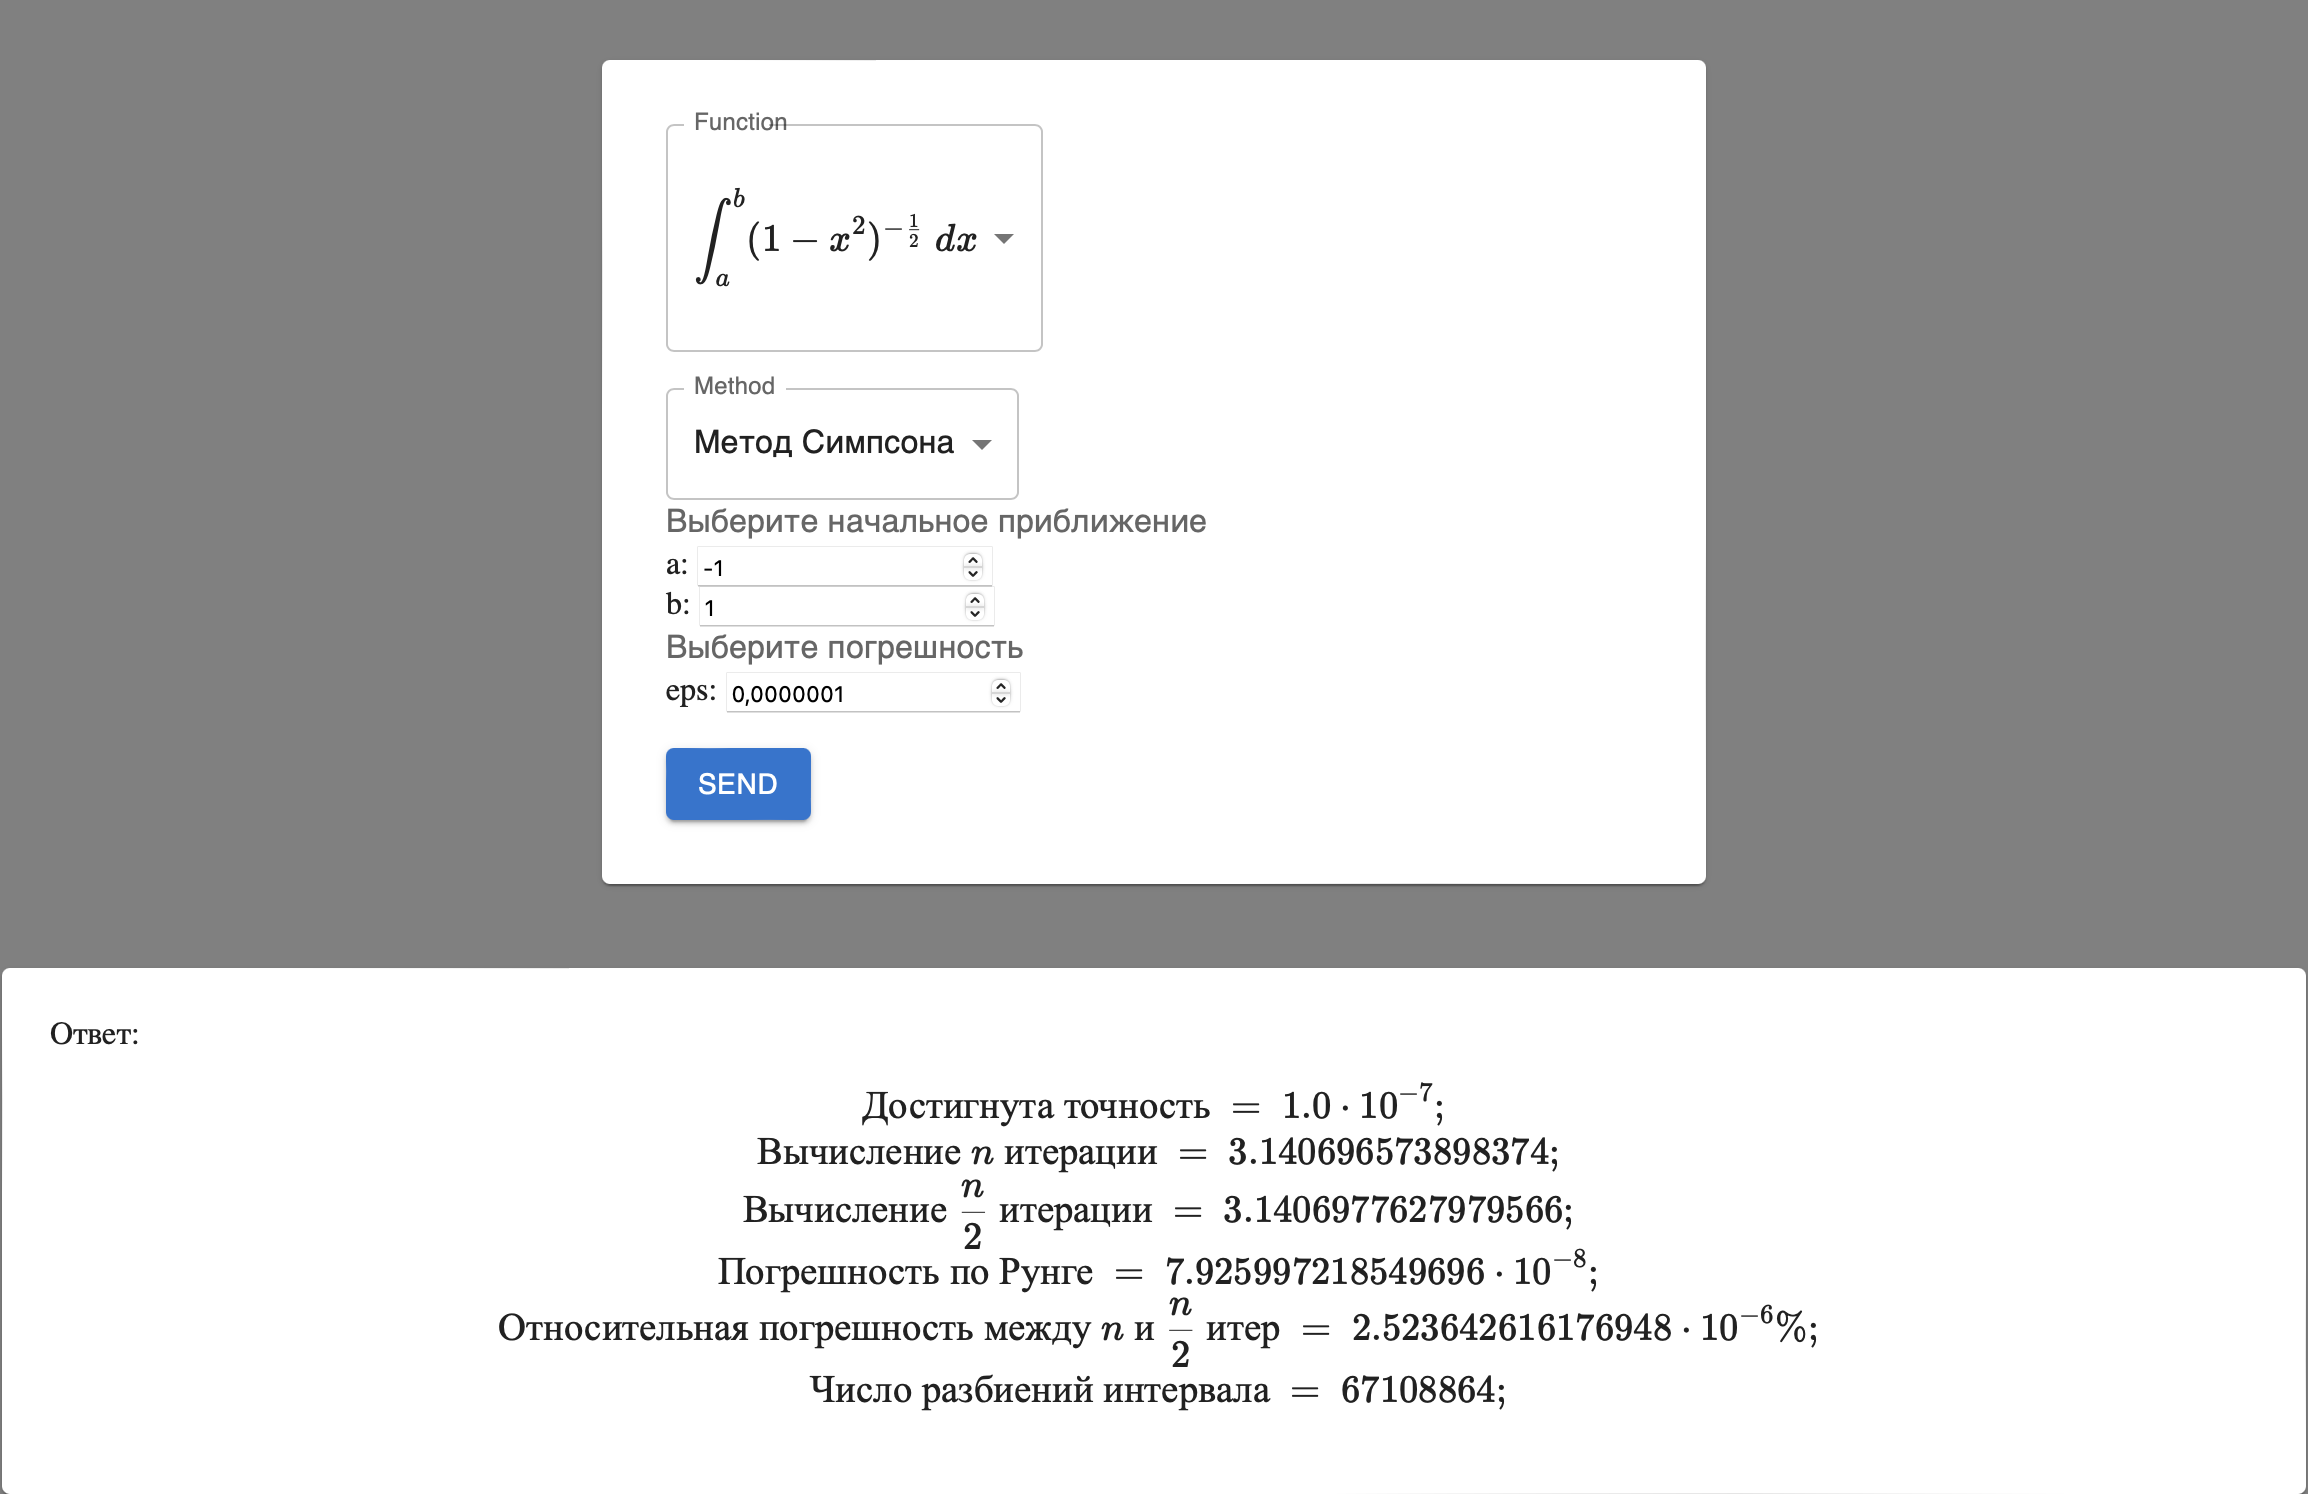
\includegraphics[width=0.9\textwidth]{example.png}
    \caption{Front: React}
    \label{fig:example}
\end{figure}

\begin{figure}[H]
    \centering
    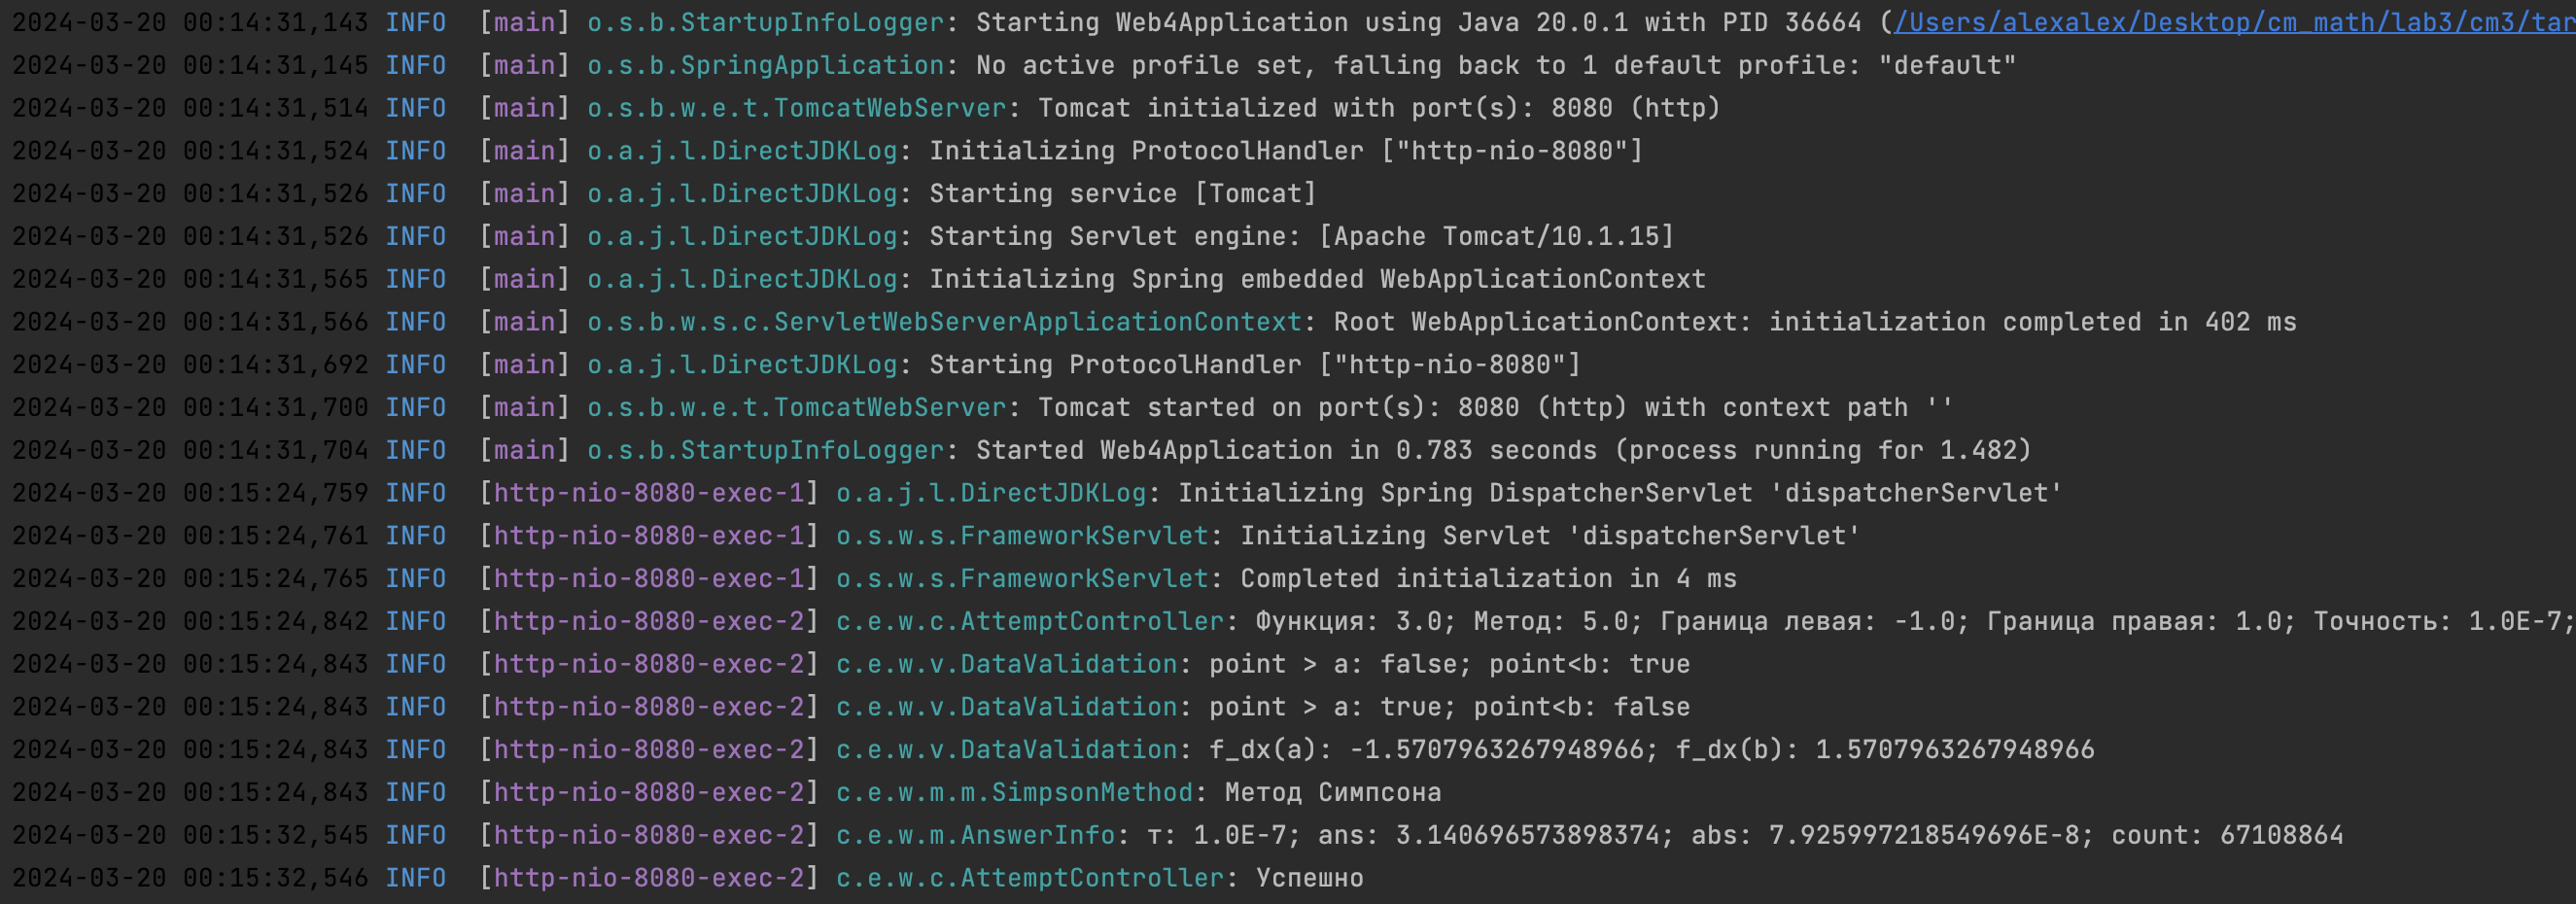
\includegraphics[width=0.9\textwidth]{logs.png}
    \caption{Backend: String logs}
    \label{fig:logs}
\end{figure}

\section{Диаграммы}

\begin{figure}[H]
    \centering
    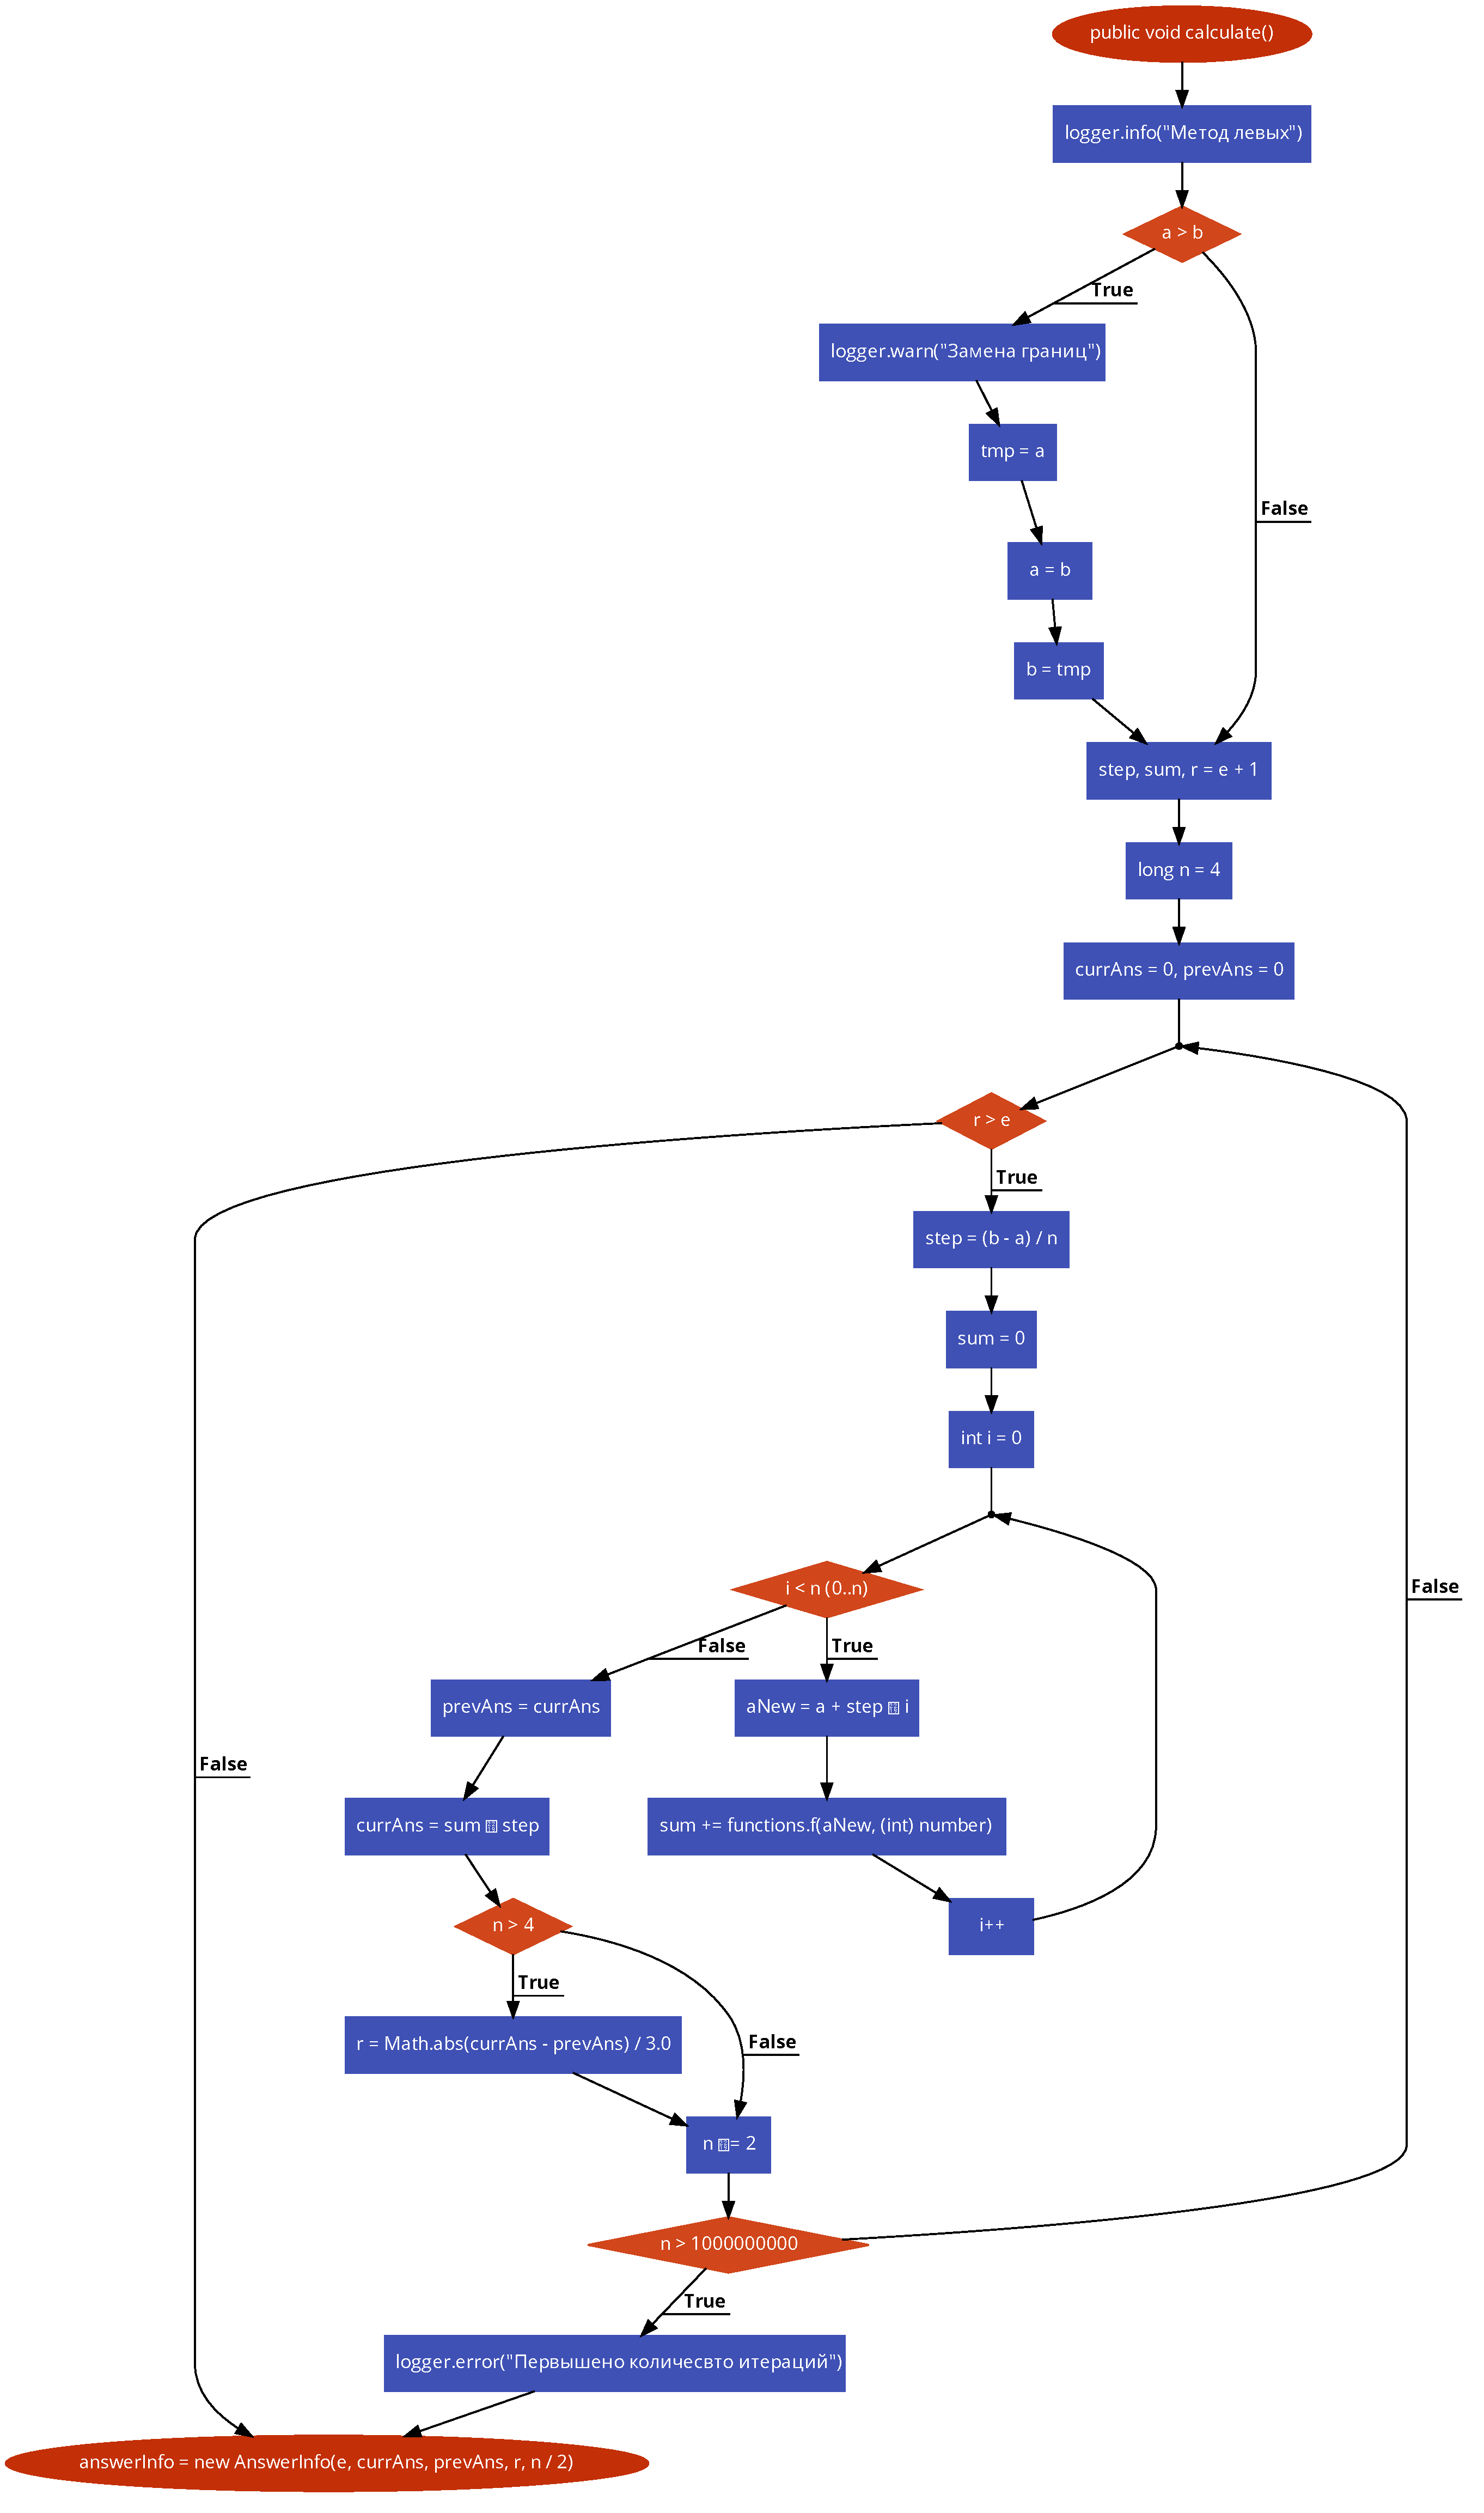
\includegraphics[width=0.5\textwidth]{left.pdf}
    \caption{Левые прямоугольники}
    \label{fig:logs}
\end{figure}

\begin{figure}[H]
    \centering
    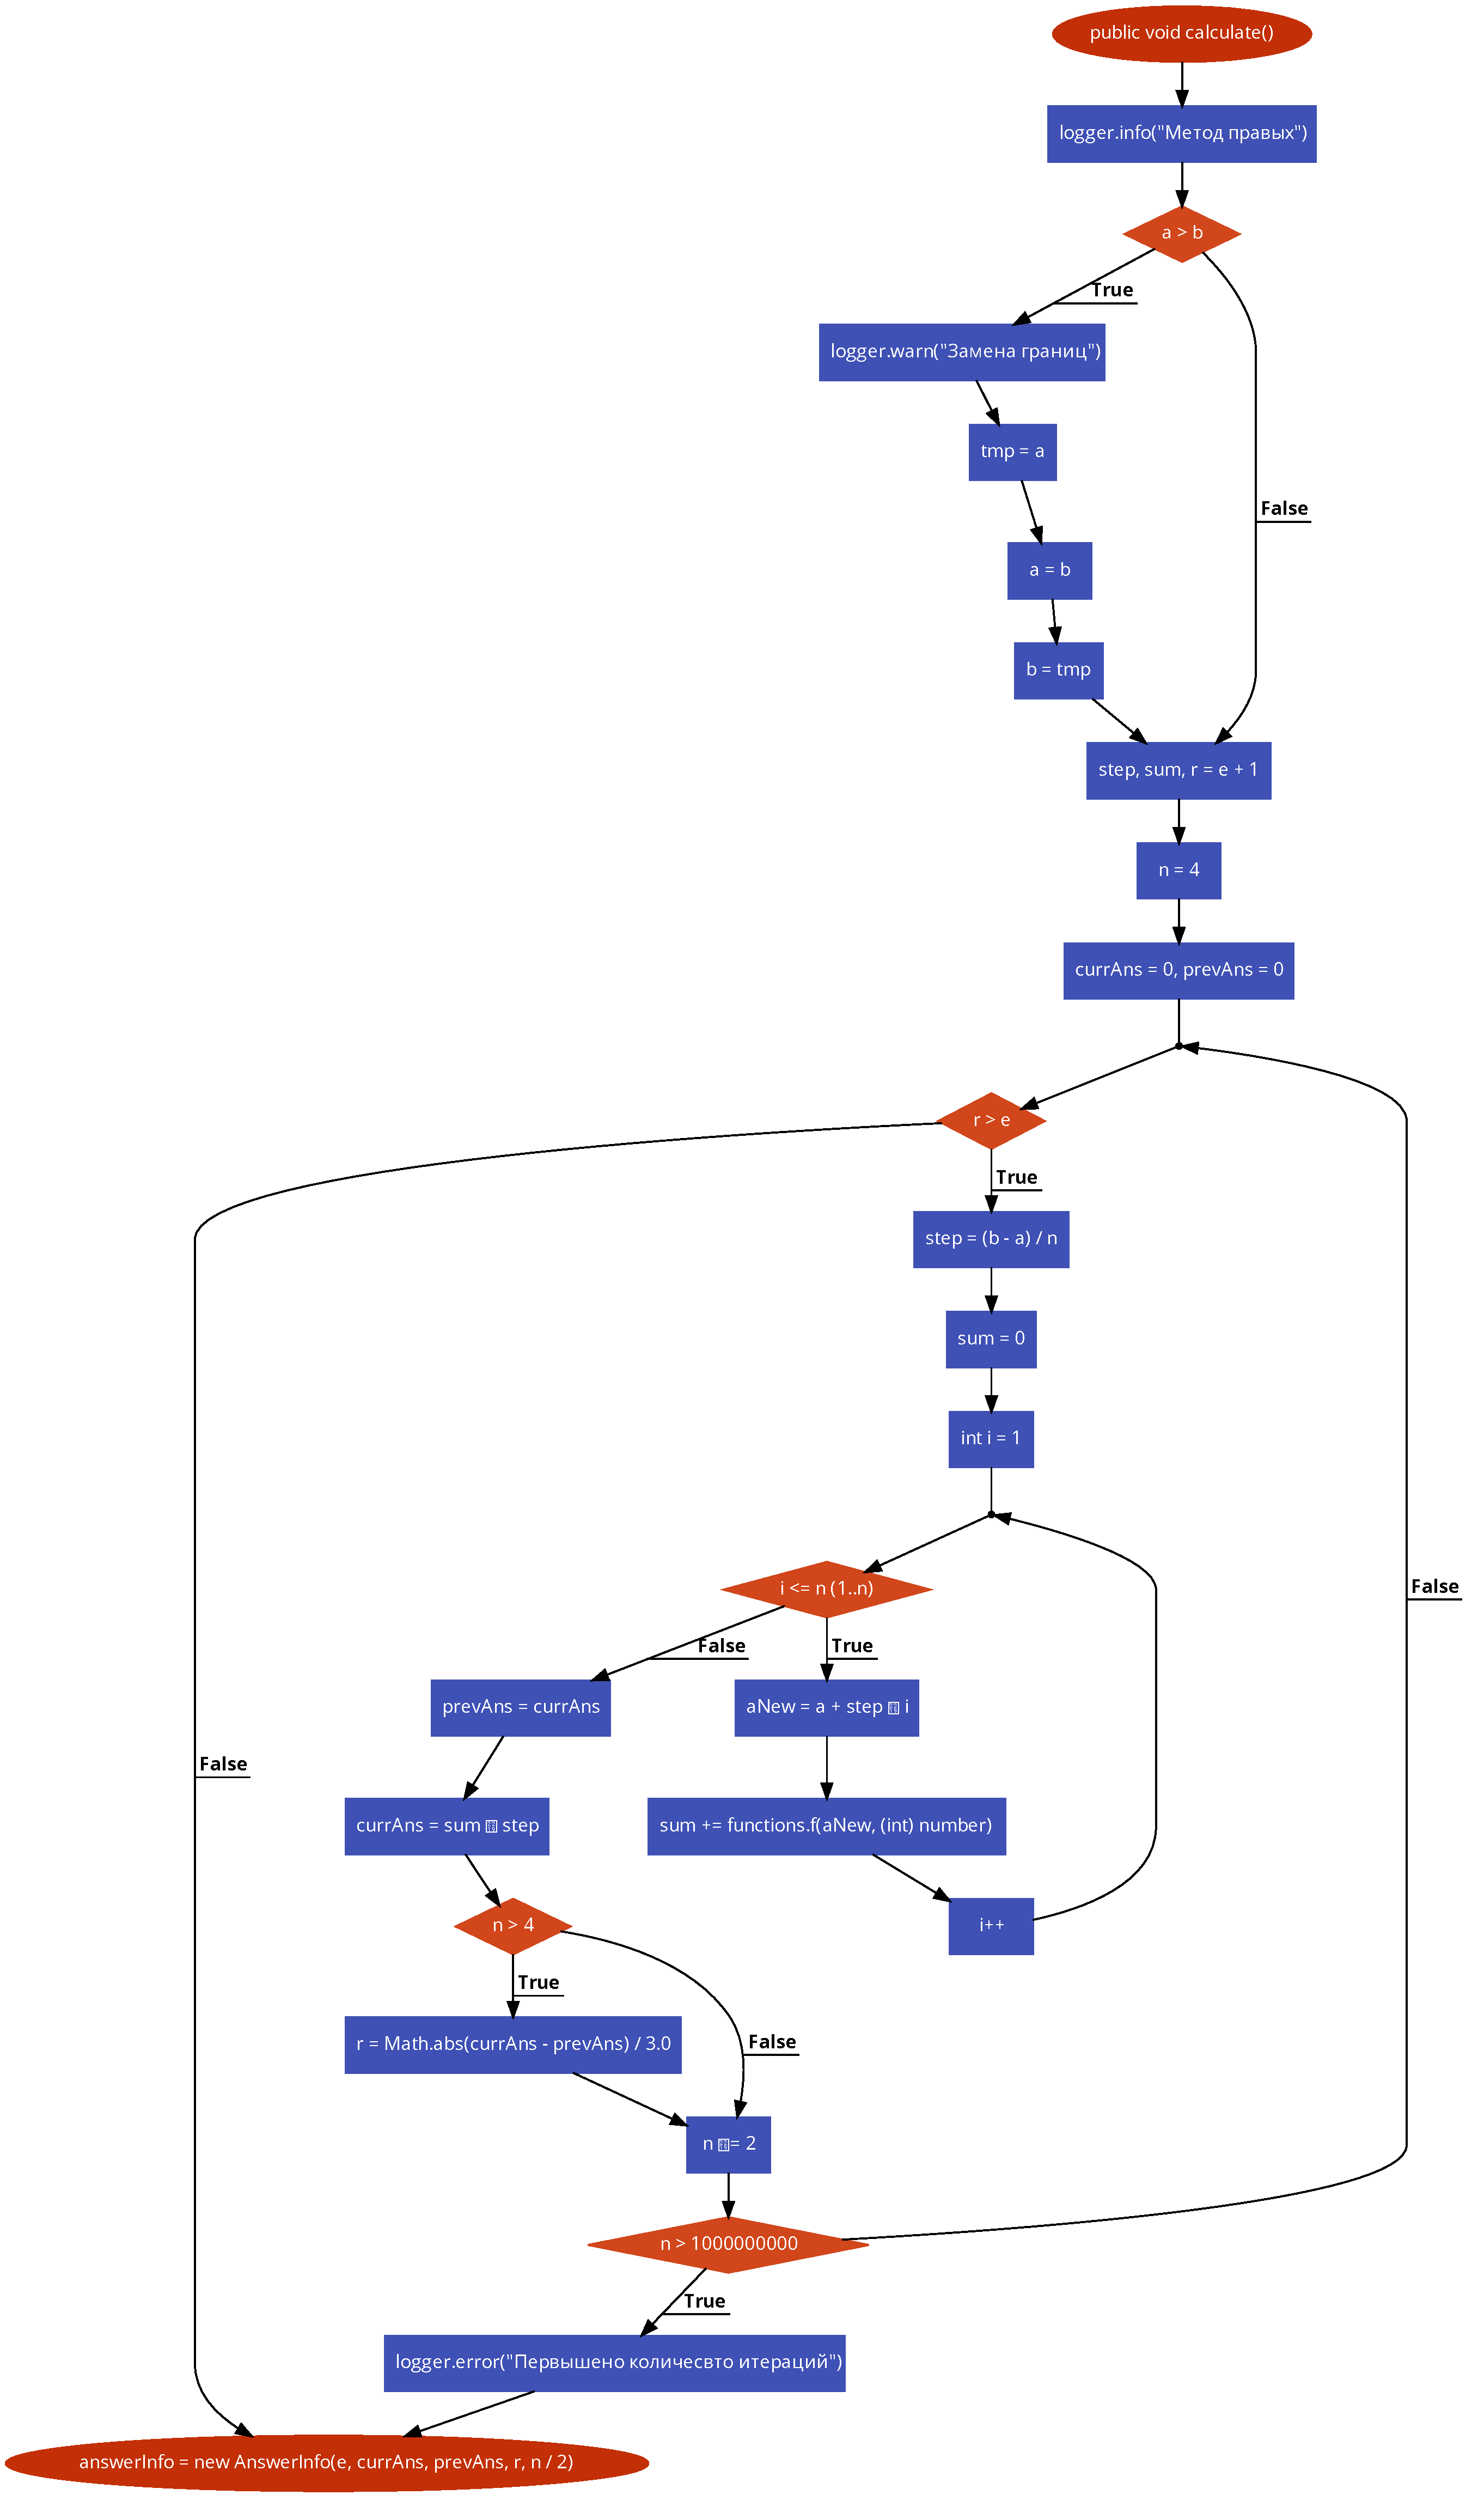
\includegraphics[width=0.5\textwidth]{right.pdf}
    \caption{Правые прямоугольники}
    \label{fig:logs}
\end{figure}

\begin{figure}[H]
    \centering
    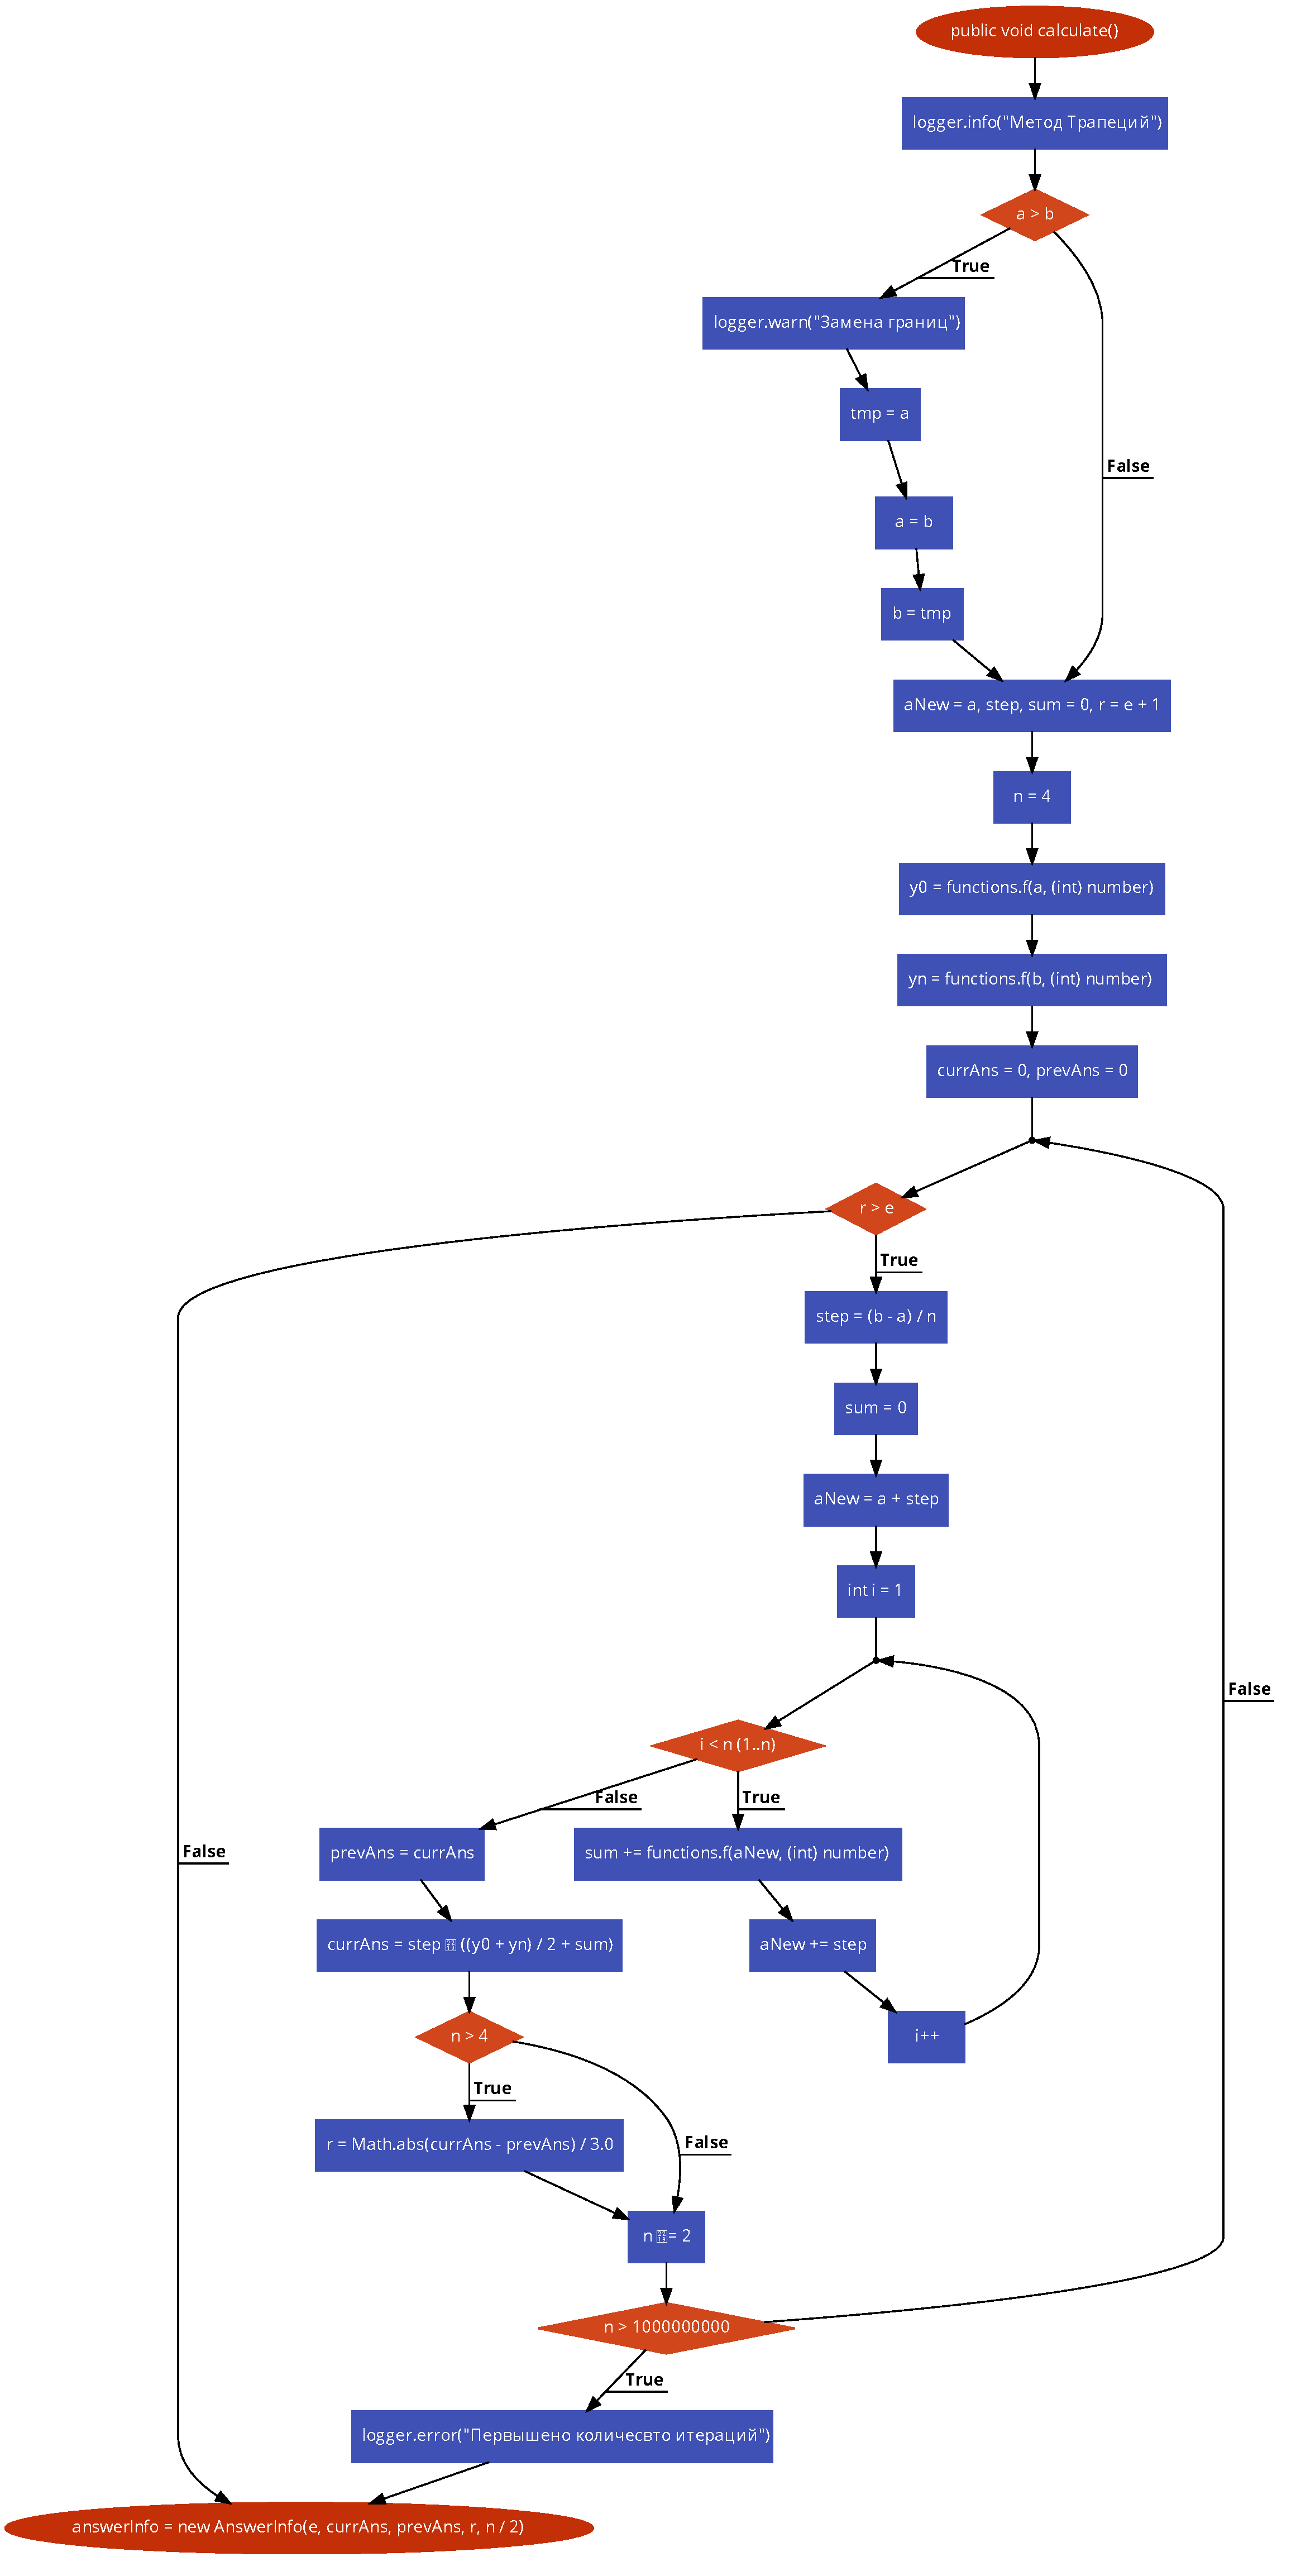
\includegraphics[width=0.5\textwidth]{trapez.pdf}
    \caption{Трапеции}
    \label{fig:logs}
\end{figure}

\begin{figure}[H]
    \centering
    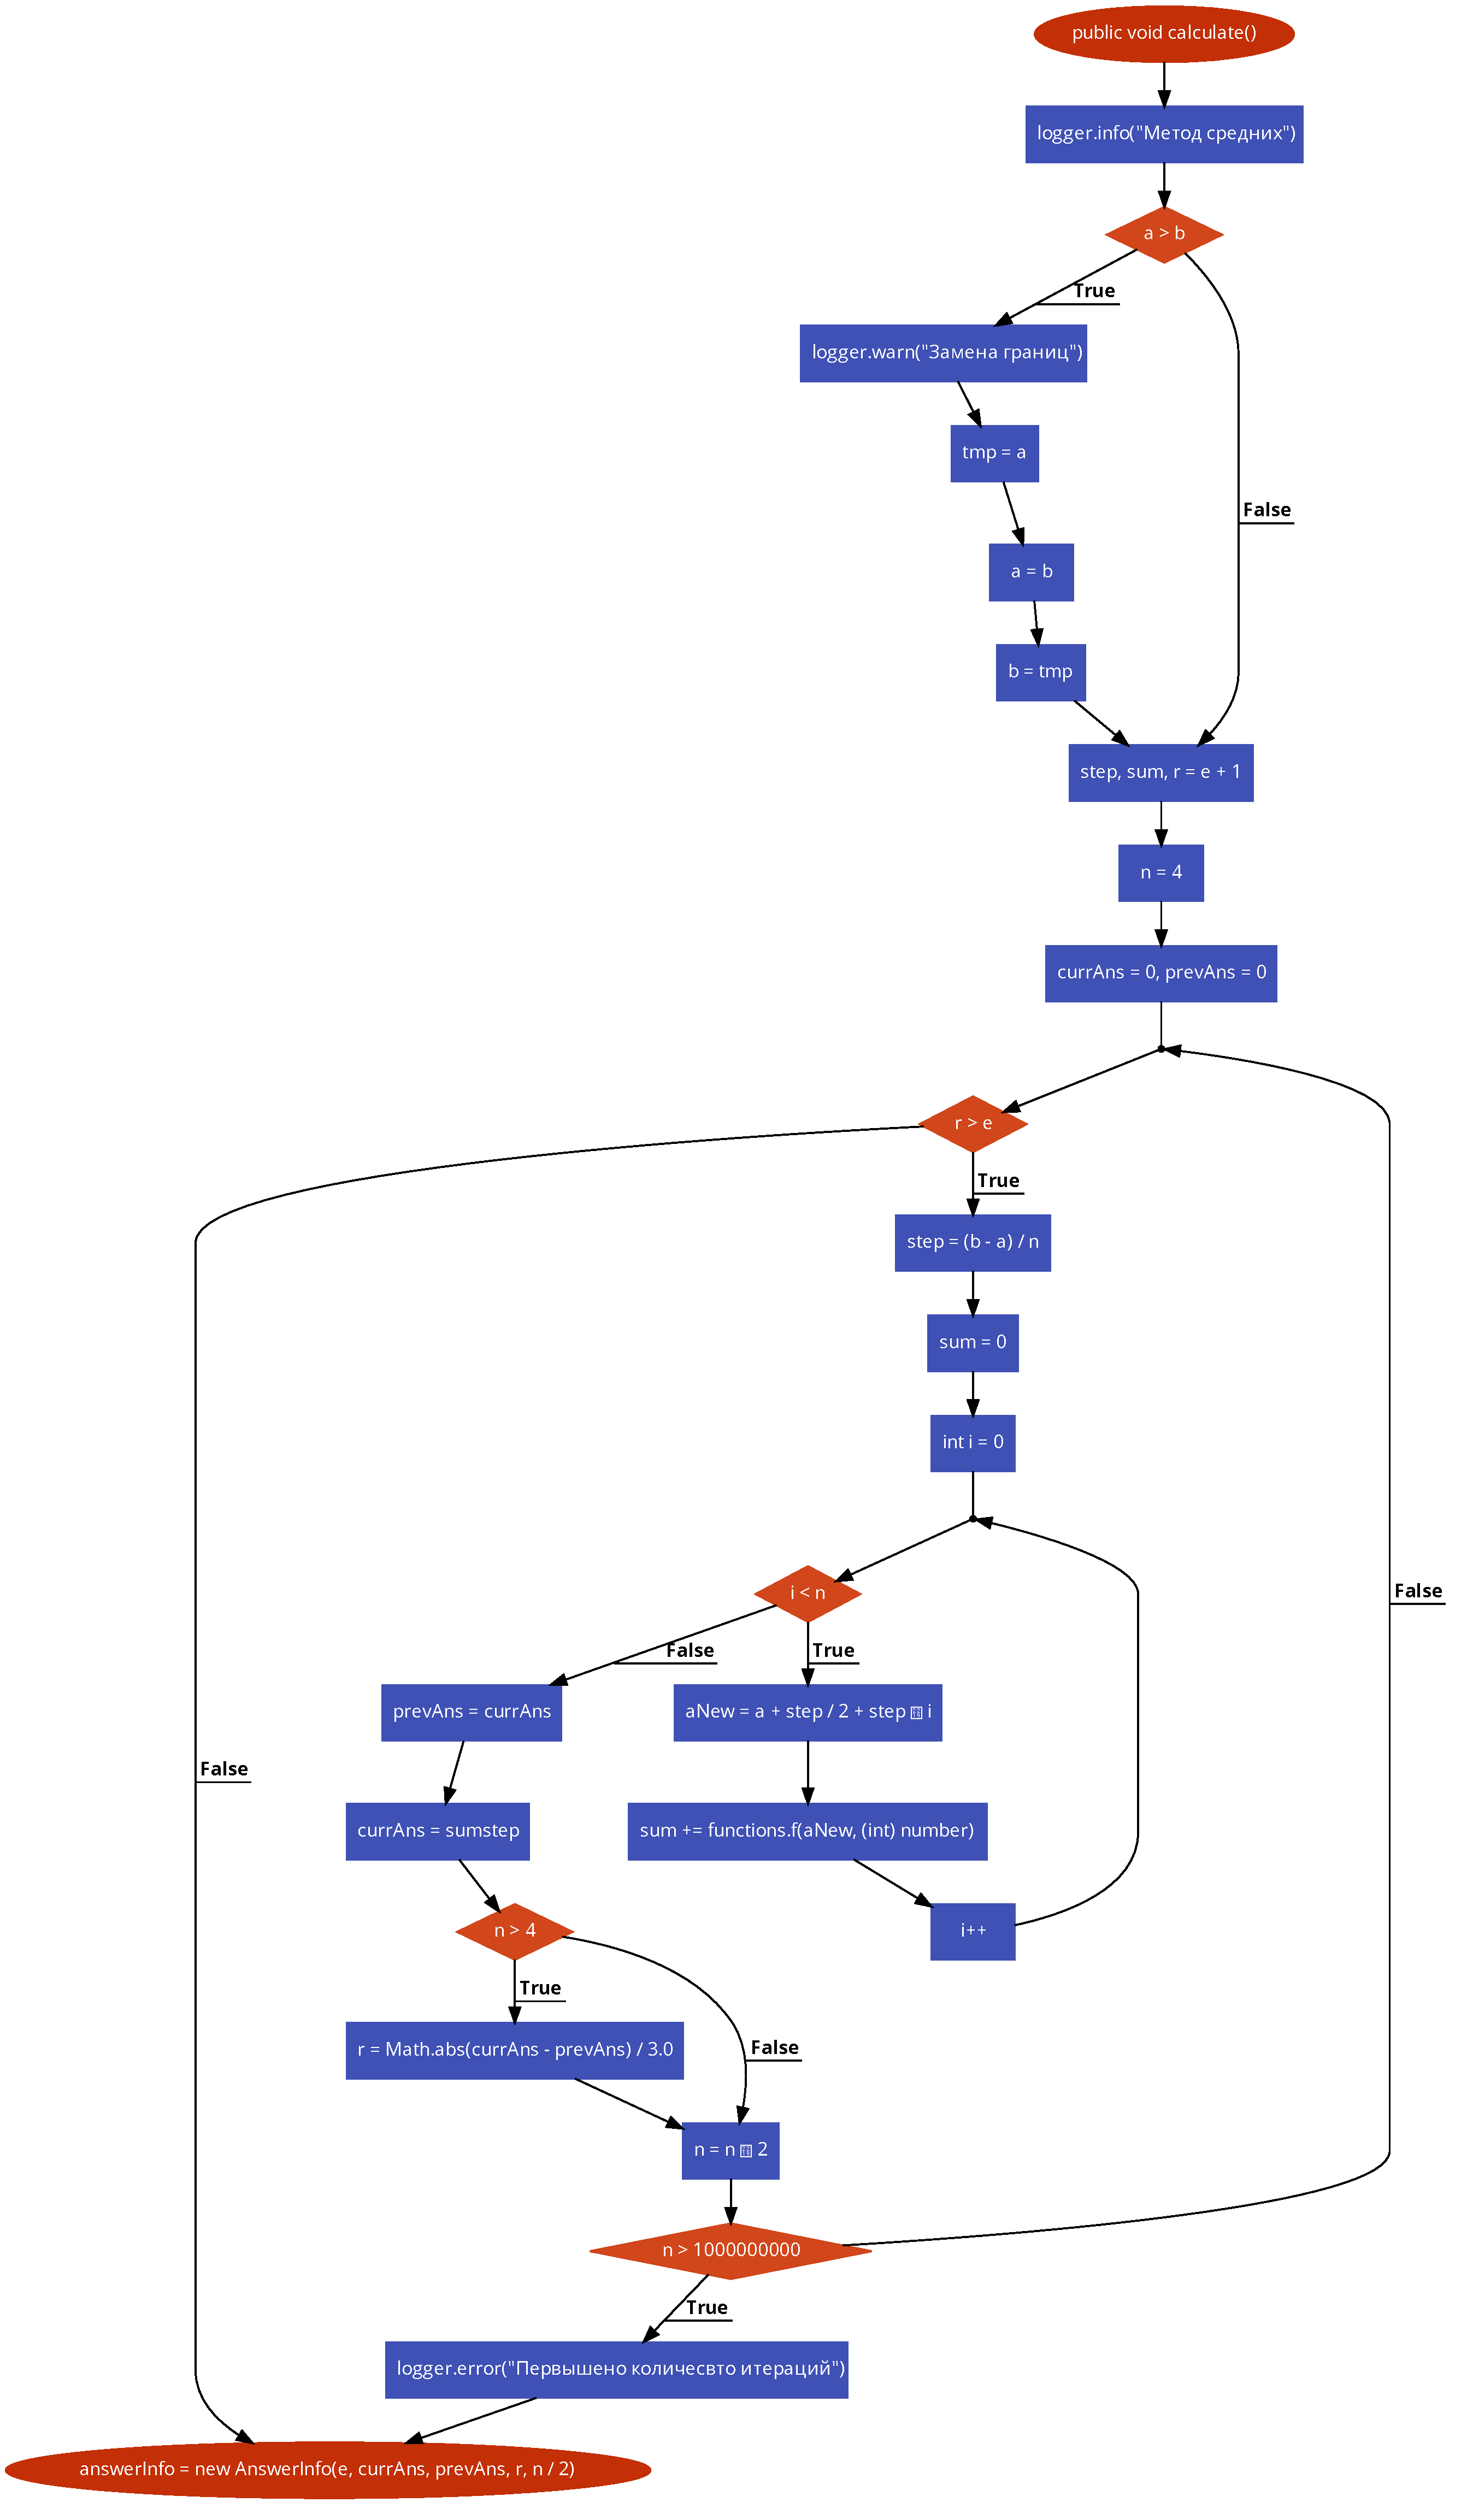
\includegraphics[width=0.5\textwidth]{center.pdf}
    \caption{Центральные прямоугольники}
    \label{fig:logs}
\end{figure}

\begin{figure}[H]
    \centering
    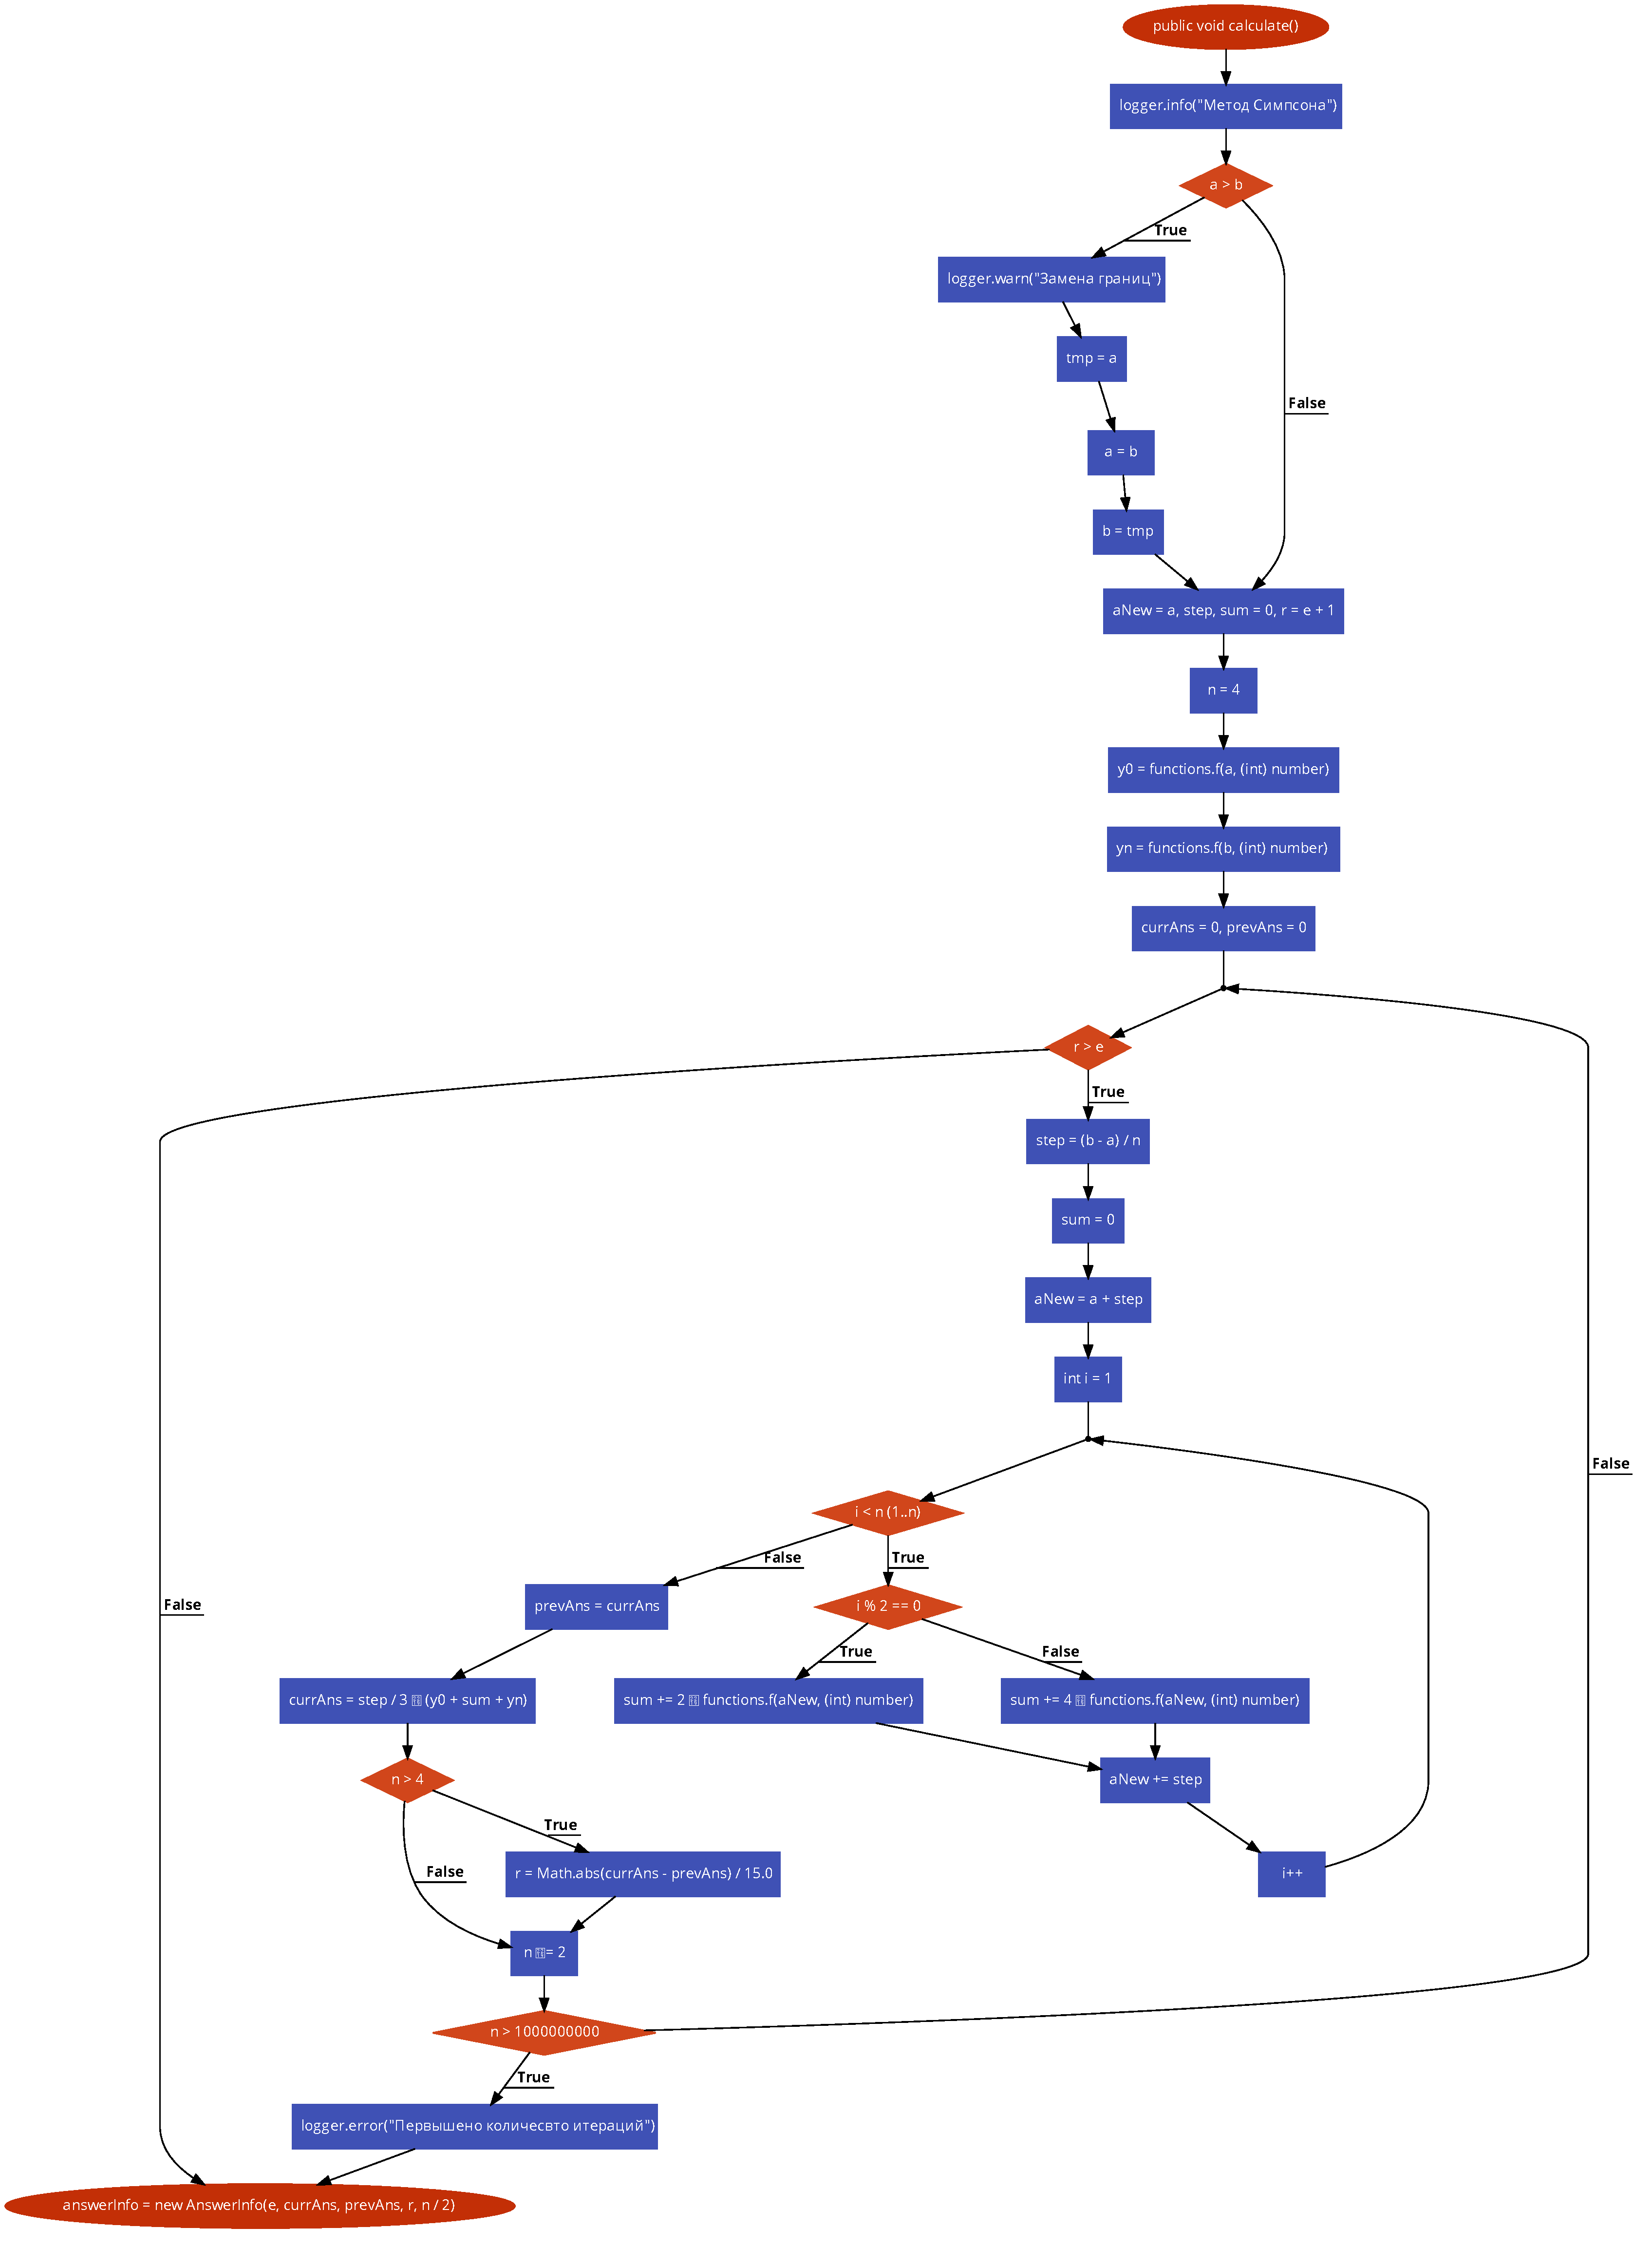
\includegraphics[width=0.6\textwidth]{simpson.pdf}
    \caption{Симпсон}
    \label{fig:logs}
\end{figure}

\section{GitHub}
Ссылка на мой репозиторий на GitHub: \url{https://github.com/Alex-de-bug/cm_math/tree/main/lab3}.

\section{Вывод}
При работе были изучены несколько численных методов вычисления интегралов, написаны несколько алгоритмов для реализации. Подсчёт руками помог усвоить все тонкости работы численных методов. Придумана обработка точек разрыва в том числе неустранимых 2го рода.
\end{document}
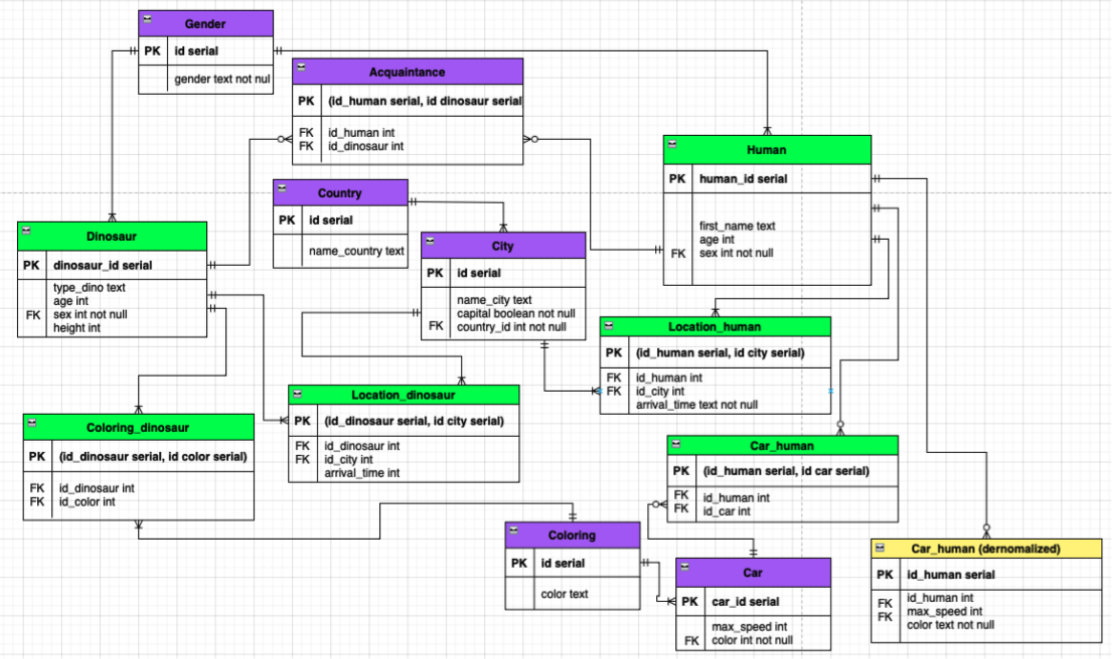
\includegraphics[width=.9\textwidth]{123}